\documentclass{mprop}

\addbibresource{../references/primary.bib}
\addbibresource{../references/secondary.bib}
\addbibresource{../references/tertiary.bib}
\addbibresource{../references/technology.bib}
\graphicspath{{../images/}}

\begin{document}

%%%%%%%%%%%%%%%%%%%%%%%%%%%%%%%%%%%%%%%%%%%%%%%%%%%%%%%%%%%%%%%%%%%
\title{Holistic Dashboard of Software Development Work-Time \& Practices}
\author{Inesh Bose}
\date{16 December 2022}
\maketitle
%%%%%%%%%%%%%%%%%%%%%%%%%%%%%%%%%%%%%%%%%%%%%%%%%%%%%%%%%%%%%%%%%%%

%%%%%%%%%%%%%%%%%%%%%%%%%%%%%%%%%%%%%%%%%%%%%%%%%%%%%%%%%%%%%%%%%%%
\tableofcontents
%%%%%%%%%%%%%%%%%%%%%%%%%%%%%%%%%%%%%%%%%%%%%%%%%%%%%%%%%%%%%%%%%%%

%%%%%%%%%%%%%%%%%%%%%%%%%%%%%%%%%%%%%%%%%%%%%%%%%%%%%%%%%%%%%%%%%%%
\newpage
\section{Introduction}

% Briefly explain the context of the research problem.

In this paper, we aim to discuss the journey of software developers as they work on projects and progress in their abilities over time; this is because \textbf{humans are the most important aspect of software engineering \cite{martinAgileSoftwareDevelopment2003}}, and we point out the frustrations that they face as they apply various disciplines to deliver reliable, efficient and high-quality products \cite{sommervilleSoftwareEngineering1992}.

\subsection{Developer Experience}

Humans interact with computers using a shared boundary between them, called an \textbf{interface}, allowing exchange of information \cite{hookwayInterface2014}, and the research of designing these interfaces is called Human-Computer Interaction (HCI) \cite{cardPsychologyHumancomputerInteraction1983}. Many times, development of any software involves evaluation of the product interface from the end-user point-of-view. However, while the end-users of a product are seen as the essential, "human" part of a system, the developers are as-important humans creating the product.

Through this project, we wish to explore more about Developer Experience (DX); using developers as the subject of study (i.e. the "human" in the Human-Computer Interaction), we understand that their interface of interacting with computers is using various tools. Most notably, the main tool can be a form of Integrated Development Environment (IDE) with the main element being the Text Editor. The purpose of this interaction is to provide a low level form of instructions to the computer, using software development, to allow end-users to interact with their tools using high-level instructions.

\subsection{Outline \& Contributions}

The contributions that this paper makes are based on the sections outlined as follows:

\begin{itemize}
    \setlength\itemsep{0.6em}
    \item \textbf{Section 2} \textit{Statement of Problem} states the problem to be addressed in the forthcoming project and explain why it is worthwhile to solve this problem;
    \item \textbf{Section 3} \textit{Background Survey} presents an overview of relevant previous work including articles, books, and existing software products, and critically evaluate the strengths and weaknesses of these works;
    \item \textbf{Section 4} \textit{Proposed Approach} shares how the planned solution aims to solve the problem outlining the feasibility and risks associated;
    \item \textbf{Section 5} \textit{Work Plan} conveys how this work would be organised with the important deliverables and carried out through the timeframe of the project.
\end{itemize}

%%%%%%%%%%%%%%%%%%%%%%%%%%%%%%%%%%%%%%%%%%%%%%%%%%%%%%%%%%%%%%%%%%%
\newpage
\section{Statement of Problem}

% Clearly state the problem to be addressed in your forthcoming project. Explain why it would be worthwhile to solve this problem.

More focus and importance is given to User Experience (UX) which can lead to lack of realisation for DX. Providing a better DX can help deliver greater UX and better productivity; hence they are directly proportional. This is what we wish to address. A project with good DX would involve usage of best practices, automation, issue tracking, robust tools that integrate into a bug-free, strong-foundation system with minimal technical debt.

\subsection{Foundations}\label{subsec:Foundations}

There are numerous APIs \& packages available for a project, especially with the drive in the open-source community. PyPI has around 420K projects with more than 4M releases \cite{PyPIPythonPackagea} and npm.js has more than 1M projects \cite{NpmBlogArchive}; these are package registries for Python and Node.js (JavaScript run-time) respectively. More than 20 million developers joined GitHub in 2022 \cite{GlobalDeveloperCommunity}. There are different systems, requirements and languages, that have their own conventions, one would need to work with (through the aid of documentation if available or it is an established package, or communities such as Stack Overflow or GitHub Discussions that have hundreds of unique use-case questions everyday, or search engines like Google to index everything on the internet related to the package).

The initial setup for any system is an important step and can mitigate majority of the frustrations from the development environment. Developers that continue development without the right foundation increase the technical debt without realising.

\subsection{Subjectivity}

In teams, there are several factors that affect each member coming from different backgrounds causing development to be highly subjective, while irrespective of team members, changes should be objective. This is seen to be very common and a major frustration point for teams of computing science students \cite{waiteStudentCultureVs2004}.

\begin{itemize}
    \item \textbf{Experience:} Individuals may have been exposed to different projects or none at all. For example, a team can have a engineer working in the industry for a couple of years making mobile applications but is put in a project for developer operations with a team of graduates and novice developers.
    \item \textbf{Passion:} They may be motivated to deliver better quality solutions or the project may not interest them. For example, a person may see opportunity to refactor legacy code to be more efficient, while another team member may not bother (and also make a valid argument to not spend time estimations on it), as \textcite{marzoloExtremeDevelopmentMeans2021} states student teams tend to develop projects with minimum efforts to pass the exam.
    \item \textbf{Beliefs:} Depending upon experience and passion, they may judge the suitability of strategies or solutions differently. For example, a member may prefer to use technologies that they are familiar and comfortable with, while others are unfamiliar but believe they know better alternatives.
\end{itemize}

\subsection{Awareness}%Visualisation

HCI focuses a lot on the importance of visualisation - humans need to be given visual feedback on their interface \cite{liCategorisationVisualisationMethods2016}. Git \cite{Git} has been very useful in change management, showing commit history and diffs over branches, and platforms such as GitHub \cite{GitHubLetBuild}, GitLab \cite{OneDevOpsPlatform}, and Bitbucket \cite{BitbucketGitSolution} (to name a few) provide additional features such as automated pipelines that can also run tests on changes and alert the developers \cite{FeaturesGitHubActionsa,GitLabCICD,atlassianBitbucketPipelinesContinuous}. There are also services, such as Codacy \cite{DevOpsIntelligencePlatforma}, Code Climate \cite{DataDrivenEngineeringIntelligence}, Libraries.io \cite{LibrariesOpenSourcea} and Snyk \cite{SnykDeveloperSecurity2020a}, that specialise in different aspects of a repository such as code quality, maintainability, dependencies and vulnerability. Dependabot \cite{Dependabot} alerted developers on GitHub and secured 18M projects in 2022 \cite{GlobalDeveloperCommunity}. Tools like Shields.io \cite{ShieldsIoQualitya} provide the ability to embed feedback images onto important documents of the project (such as README.md). However, there is still a lack of an intuitive method of revealing their habits, and this could be very useful in reminding developers about the state of their project.

\begin{figure*}[h]
    \captionsetup{labelformat=empty}
    \centering
    \begin{subfigure}[b]{0.475\textwidth}
        \centering
        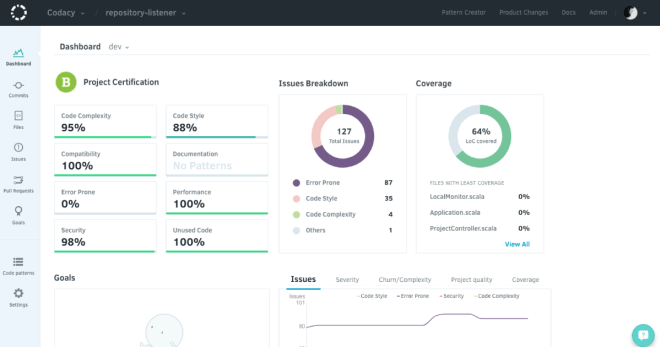
\includegraphics[width=\textwidth]{codacy_dashboard.png}
        \caption[]%
        {{\small Codacy}}
    \end{subfigure}
    \hfill
    \begin{subfigure}[b]{0.475\textwidth}  
        \centering 
        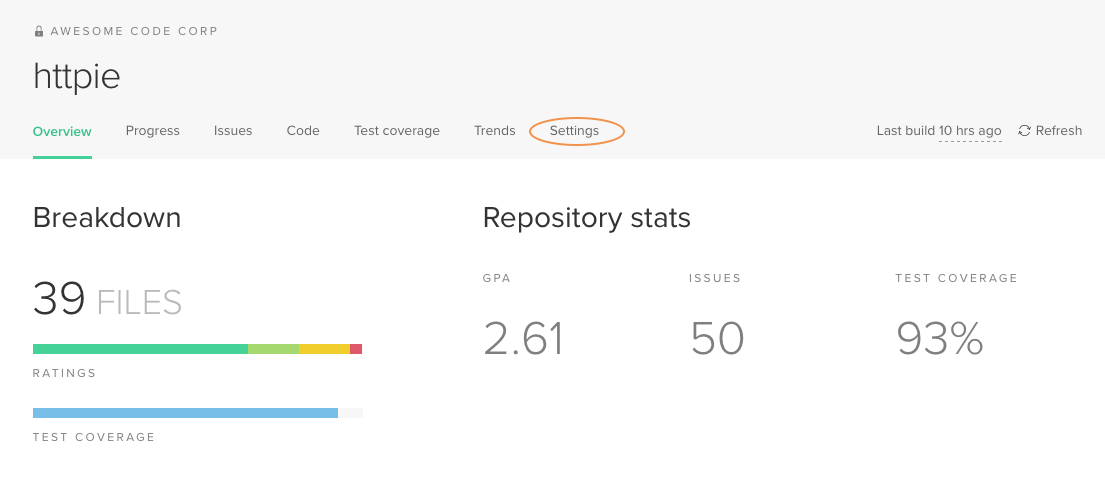
\includegraphics[width=\textwidth]{codeclimate_dashboard.png}
        \caption[]%
        {{\small Code Climate}}
    \end{subfigure}
    \vskip\baselineskip
    \begin{subfigure}[b]{0.475\textwidth}   
        \centering 
        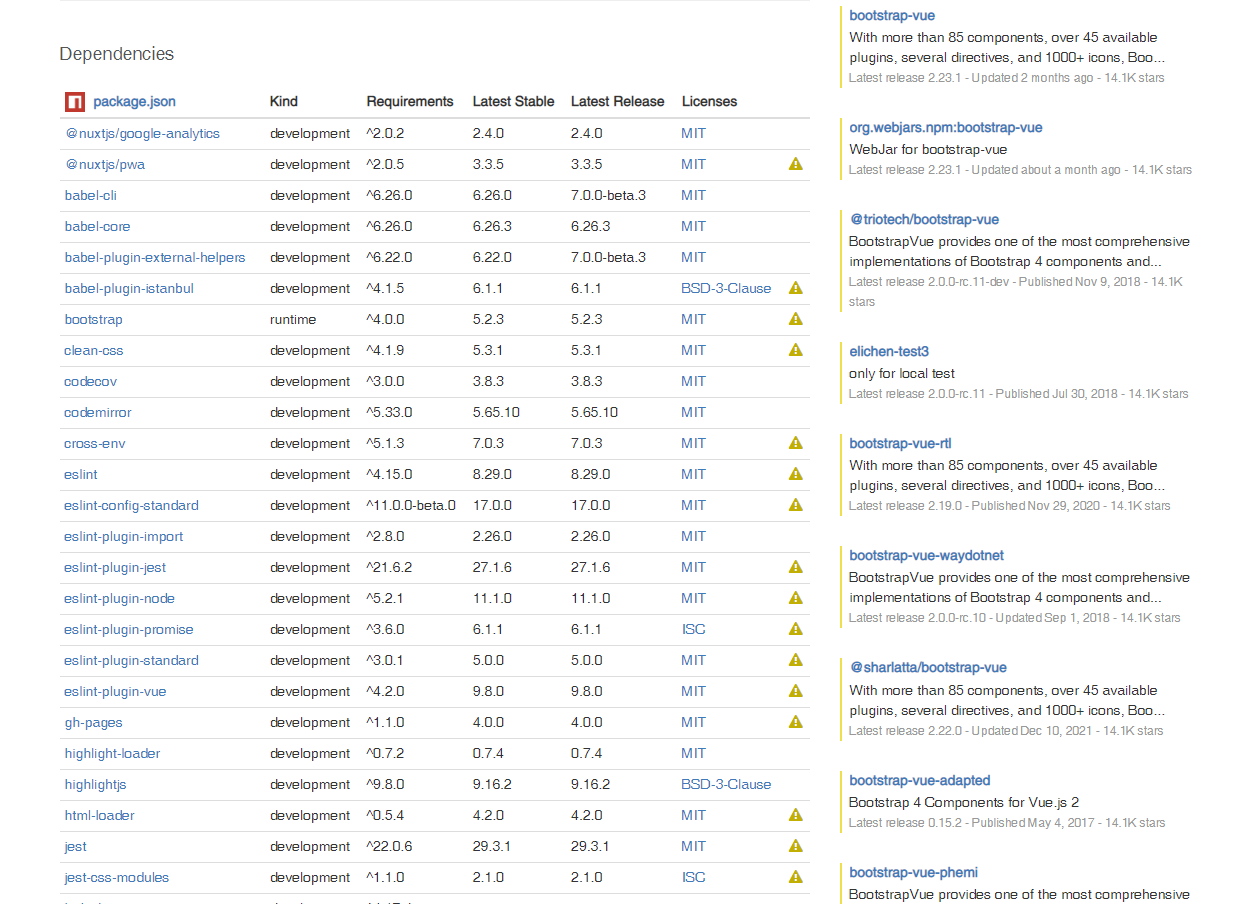
\includegraphics[width=\textwidth]{librariesio_dashboard.png}
        \caption[]%
        {{\small Libraries.io}}
    \end{subfigure}
    \hfill
    \begin{subfigure}[b]{0.475\textwidth}   
        \centering 
        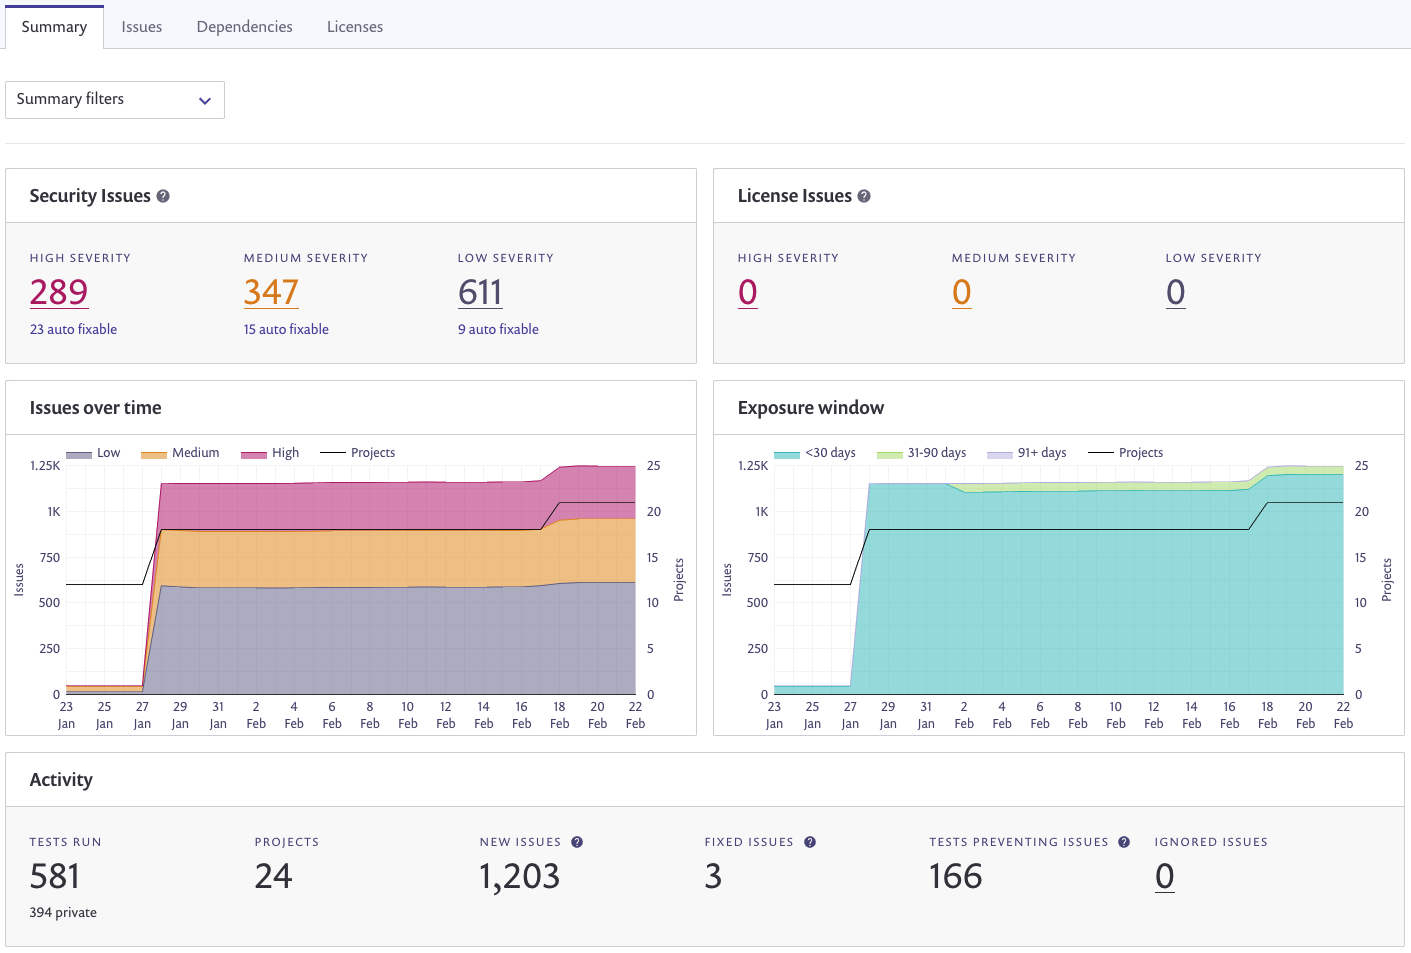
\includegraphics[width=\textwidth]{snyk_dashboard.png}
        \caption[]%
        {{\small Snyk}}
    \end{subfigure}
    \caption[]
    {\small Dashboards for different code monitoring services} 
\end{figure*}

%%%%%%%%%%%%%%%%%%%%%%%%%%%%%%%%%%%%%%%%%%%%%%%%%%%%%%%%%%%%%%%%%%%
\newpage
\section{Background Survey}

% Present an overview of relevant previous work including articles, books, and existing software products. Critically evaluate the strengths and weaknesses of the previous work.

This section reveals and discusses the literature review, of the established, related works, conducted by categorising search into areas relevant to developers.

\subsection{Productivity}

In current times, we have seen systems modernising and software growing rapidly and being delivered really fast. Recent significant examples include Zoom and Microsoft Teams over the COVID-19 Pandemic, providing new features and bugfixes at an incredible speed as the demand grew exponentially. In such circumstances, companies aim to improve their process efficiency and employ developers with high productivity (a reflection of this in many job postings that include the test "ability to move in a quick environment"); hence they tend to measure software productivity \cite{devanbuAnalyticalEmpiricalEvaluation1996}. While productivity is defined as the ratio between the number of outputs (such as bugfixes \& features implementation) over the number of inputs (such as time) \cite{morisioFrameworkBasedSoftware1999,pritchard1995productivity}, it is difficult to contrast this definition to software development where, compared to industrial productions involving repeating processes, software organisations typically develop new solutions \cite{trendowiczChapterFactorsInfluencing2009}, but many organisations still use the simplified definition of productivity \cite{careyImpactCommunicationMode1997} - most typically source lines of code (SLOC) per work-month \cite{barry1981software,conteSoftwareEngineeringMetrics1986,jonesProgrammingProductivity1985}. It can be much more complex than that.

We've established the steps software engineering involves along with the complexities of developers - it is not a linear path \cite{abdel-hamidSlipperyPathProductivity1996,briand2002software,kemererEmpiricalValidationSoftware1987}. Some automated process metrics used are: lines of source code (SLOC) written \cite{devanbuAnalyticalEmpiricalEvaluation1996,walstonMethodProgrammingMeasurement1977}, function points \cite{albrecht1979measuring,computerstaffSoftwareMetricsGood1994}, and changes request fulfilled \cite{cataldoSociotechnicalCongruenceFramework2008,millerHowWasYour2021}; but these are highly objective and may only capture a small part of developer's work. Research has been carried to understand developer productivity and its influencing factors under different contexts; \textcite{trendowiczChapterFactorsInfluencing2009} lists these based on over a hundred publications along with their experiences involving industrial projects, workshops and surveys on software productivity, eventually learning that productivity of software development processes would depend significantly on the capabilities of the developers along with the tools and methods that they use; \textbf{the first step of quantifying productivity management is selecting the right metrics}.

A major reason why companies wish to measure productivity is cost reduction. According to \textcite{boehmImprovingSoftwareProductivity1987}, \$140 billion is spent annually worldwide on software (this is 35 years ago and the number is expected to be much larger than this now). The metrics could be helpful in understanding how resources are being used and to predict if a project would succeed. \textcite{mockusSuccessionMeasuringTransfer2009} measured productivity based on successful deliveries in a project, however the study could not be applied to contexts with different definitions of "success".

More appropriate to large projects is to have experienced developers in their core team, hence \textcite{gillProductivityImpactsSoftware1990} looked at how productivity could be related to experience and found that software engineers with more experience were more productive, but using resources to recruit such engineers revealed declining marginal returns; instead, putting greater emphasis on the design phase of a project is associated with increased productivity.

Within teams, however, productivity is much different than for individuals \cite{kimUnderstandingPersonalProductivity2019,markNeuroticsCanFocus2016}. Moreover, despite measuring productivity using the right metrics, the perception of productivity is highly subjective \cite{koWhyWeShould2019,meyerSoftwareDevelopersPerceptions2014}. \textcite{lakhanpalUnderstandingFactorsInfluencing1993} found team cohesion to be the dominating factor when investigating team performance, but this was using a one-time survey. \textcite{canedoFactorsAffectingSoftware2019} revealed 37 factors to be pertinent to team productivity including individual characteristics such as work experience \cite{deomeloInterpretativeCaseStudies2013} and skill/competence \cite{maxwellBenchmarkingSoftwareDevelopmentProductivity2000,oliveiraSoftwareProjectManagers2016}, while there's also collaboration \cite{clincySoftwareDevelopmentProductivity2003,stephanidisHCIInternational20152015}, team member availability \cite{deomeloInterpretativeCaseStudies2013,maxwellBenchmarkingSoftwareDevelopmentProductivity2000}, and ease of communication \cite{wagnerSystematicReviewProductivity2018,yilmazEffectiveSocialProductivity2016}. \textcite{ruvimovaExploratoryStudyProductivity2022} carries out a study in a practical environment with 25 individuals across five software teams reporting their perceived productivity for themselves and their team over interviews and surveys, and the most important finding from their study was realising that teams in modern organisations are highly fluid varying in size, members, structure and projects causing different aspects and dependencies to productivity.

\subsection{Learning}

Experience and knowledge of tools is a big contributing factor to productivity \cite{gillProductivityImpactsSoftware1990,deomeloInterpretativeCaseStudies2013,maxwellBenchmarkingSoftwareDevelopmentProductivity2000,oliveiraSoftwareProjectManagers2016}. After the discussion in \ref{subsec:Foundations}, we can say there are many tools that one can continue learning, and it is common for a developer to make a search as the first step. \textcite{baoTrackingAnalyzingCrossCutting2015} found that there are more than 20 queries made by developers everyday related to their development. A lot of it depends on the phase, such as requirement analysis where they search for explanation of terminologies, books and tutorials to understand business logic, or development phase where they look for third party libraries, or maintenance looking for bugs that are commonly faced hopefully with a solution provided. Understanding queries would also help understand developers' problems during the development process, to also possibly develop tools to help them (tools are available now such as IDE extensions giving links, or GitHub autopilot). \textcite{simArchetypalSourceCode1998,stoleeSolvingSearchSource2014,sadowskiHowDevelopersSearch2015,bajracharyaMiningSearchTopics2009,bajracharyaAnalyzingMiningCode2012,xia2017developers} investigate how developers make search queries for their tasks, revealing different dimensions of search along with corresponding frequencies in order to highlight the importance of developing domain-specific search engines, automated generation and refinement of search queries and knowledge sharing; many of these solutions exist in a form, like Stack Exchange.

Learning experience is also important, and some methods may not be as welcoming to learners since they come from different backgrounds. Documentation may be too technical and assumes prior knowledge, or Stack Overflow may be gate-kept \cite{cheriyan2017norm,miller2022did} (but there are reasons to instead push developers to research more instead of directly consulting help). Since providing help, writing documentation and producing tutorials requires effort, \textcite{kafer2017best} compares (passive) text-based tutorials with video-based tutorials and understand which is better in terms of efficiency and learning; they discovered negligible differences in terms of efficiency for either approaches despite each having their own sets of advantages and disadvantages  \cite{alexanderUsabilityPrintOnline2013,devaney2009impact,payneAnimatedDemonstrationsExploratory1992}. Text tutorials were completed faster \cite{mestreStudentPreferenceTutorial2012}, while video tutorials (more preferred by the participants when offered a choice) helped faster learning over the compartively longer period \cite{baeckerShowingInsteadTelling2002,lloydScreencastTutorialsEnhance2012,vandermeijComparisonPaperbasedVideo2014}. Furthermore, \textcite{begelNoviceSoftwareDevelopers2008} studies new recruits (novices) at a large organisation (Microsoft) to understand how they progress and transition to experts, finding that onboarding processes are tailored for this purpose and involve effective methods such as mentoring and pair-programming in the team.

\textcite{cockburnCostsBenefitsPair2001} reveals that many tool discovery occurs during pair programming and \textcite{murphy2011peer,murphy-hillHowUsersDiscover2015} looks into "social solutions" that allow developers to be aware of new tools. \textcite{marzoloExtremeDevelopmentMeans2021} outlined a course and used tools to monitor students learning Agile methodologies. Several research has found the lack of knowledge as a factor for a task \cite{grossmanSurveySoftwareLearnability2009} and in many cases, there is often a huge difference in developers knowing all the features that their IDE may offer \cite{campbellDesigningRefactoringTools2008}. There are notifications or alert messages such as "tip of the day" that attempt to provide awareness, but they can be seen as a bad UX step as well (depending on how the system implements it, for example if its an additional blocking step).

Using Expectation Confirmation Theory (ECT), \textcite{raufPerceivedObstaclesNovice2016} identified the obstacles novice developers may face while adopting new APIs and tools, contrary to \textcite{roehm2012professional} understanding skilled developers comprehending new tools by simply putting themselves in the role of end users of the API and avoid reading the code or documentation (developers are lazy afterall). Additionally, \textcite{murphy2019developers} reveals how learning is carried out at Google's toilets (a technique called "Testing on the Toilet") by posting 1-page newsletters about tools on the stalls; there are aspects such as requirement use-cases of the tools and memorability of the tool name that effect learning more about it.

\subsection{Experience}

Contrary to the skill-experience that developers have from the past, developer experience is about involvement in the present \cite{fagerholmDeveloperExperienceConcept2012}. If there would be no blockers on productivity, humans feel good when productive \cite{WhyDoesProductivity,beechamMotivationSoftwareEngineering2008,graziotinFeelingsMatterCorrelation2015,amabileProgressPrincipleUsing2011,meyerSoftwareDevelopersPerceptions2014,mullerStuckFrustratedFlow2015,khanMoodsAffectProgrammers2011}. A lot of papers in the previous sections have also considered learning experience, along with frustration of using tools if there is no knowledge of it. Many solutions and tools are factoring-in developer experience in their priorities. \textcite{StackOverflowDeveloper} reveals the most loved and dreaded programming languages (Rust and COBOL respectively), and JavaScript frameworks such as Svelte \cite{SvelteCyberneticallyEnhanced} and Nuxt \cite{NuxtIntuitiveWeb} (SSR Vue) provide many features to improve developer experience \cite{StateJS2021}.

Significant specialised research has not yet been conducted, but it is well-established at this point that human factors are the most important aspects to intellectual software development \cite{endresHandbookSoftwareSystems2003}, in terms of performance \cite{sackmanExploratoryExperimentalStudies1968,demarcoProgrammerPerformanceEffects1985} and quality \cite{mockusOrganizationalVolatilityIts2010,trendowiczChapterFactorsInfluencing2009,birdPuttingItAll2009,nagappanInfluenceOrganizationalStructure2008}. Many articles provide various definitions for DX, but also consider the developer journey and provide methods of improving DX (such as providing documentation, communication, utilities) since it is realised to be an important area for software engineering \cite{fagerholmDeveloperExperienceConcept2012,DeveloperExperienceDevEx,cavalcanteWhatDXDeveloper2021,doerrfeldWhatDeveloperExperience2022,WhatDeveloperExperience}. \textcite{GoodDeveloperExperience} expands the Project Management / Quality Triangle (created by Barners in 1980) \cite{ProjectManagementTriangle,ProjectTriangleMicrosoft} showing the relationship between "Time", "Money" and "Scope" to a Pyramid having "Emotional Cost" as the last corner.

\subsection{Structure}%(Individual \& Teams)

Development is also influenced by the structure of the process - it can involve working individually or in a team. Productivity is perceived differently in teams (like tasks depending on others' availability) \cite{ruvimovaExploratoryStudyProductivity2022}, and learning can also take place in a team (pair programming) \cite{murphy2019developers}. \textcite{cookeMeasuringTeamKnowledge2001,lewisMeasuringTransactiveMemory2003} view teams as a primary mechanism for leveraging specialised knowledge, and so a software team is staffed according to distribution of knowledge of tools required for a successful completion of a project \cite{walzSoftwareDesignTeam1993}. Having only individuals with diverse knowledge is an insufficient condition to achieve quality performance in a software project \cite{farajCoordinatingExpertiseSoftware2000}. Lack of trust, difficulties in communication, and lack
of identification with project goals negatively impact the
success of projects \cite{smiteEmpiricalEvidenceGlobal2010,holmstromAgilePracticesReduce2006,hymanCreativeChaosHighperformance1993}.

\textcite{basili1979investigation} found relationships between the size of a programming group and several software metrics. Group structures were outlined as Chief Programmer Team by \textcite{mills1971chief,bakerChiefProgrammerTeam1972} and Egoless Programming Team by \textcite{weinbergPsychologyComputerProgramming1988}, and \textcite{manteiEffectProgrammingTeam1981} compares these two structures for managing programming projects and classified performance based on task properties such as difficulty, size, duration, modularity, reliability, time and sociability; it was revealed that a hybrid model (Controlled Decentralised) team is highly effective. Similarly, \textcite{sawyerSoftwareDevelopmentTeams2004} focuses on ways software developers organise information and discuss the archetypes of software development teams (Sequence, Group, and Network) and discovering hybrid models to be good solutions. Other factors revealed by \textcite{heTeamCognitionDevelopment2007} are frequency of meetings having positive affects on team cognition while emails had no effect, along with gender diversity strongly affecting cognition positively.

In evaluating team structures, \textcite{amritIdentifyingCoordinationProblems2012} sought for coordination problems in teams using analysis tools and finding it difficult to quantify clashes accurately. \textcite{lopez-fernandezDevOpsTeamStructures2022} studied DevOps teams and classified them based on variables such as collaboration frequency, product ownership sharing, and autonomy, while \textcite{nanJointEffectTeam2013} aimed to understand open-source collaboration revealing that performance is directly proportional on size \& structural interdependency.

\subsection{Practices}

Experienced developers are aware of many tools, but they can still discover new ones \cite{murphy2011peer,murphy-hillHowUsersDiscover2015}. There are tools available to measure productivity, code health, etc. \textcite{lajiosSoftwareMetricsSuites2009} attempts to determine individual metric suites, that fit projects without correlating too highly with each other for quality assessment and defect prediction, using machine learning and applying Correlation-based Feature Selection (CFS), and learnt that Lines of Code and WMCMcCabe were the most commonly suited metrics with no CK metrics seen. \textcite{blondeauSoftwareMetricsPredict2015} distinguishes metrics that would be useful to evaluate the status of a project by carrying a literature review and evaluation of a project at a major IT company. They learnt that metrics highly depend on the project and that there are separate benchmarks and understanding of customer requests for each project.

%%%%%%%%%%%%%%%%%%%%%%%%%%%%%%%%%%%%%%%%%%%%%%%%%%%%%%%%%%%%%%%%%%%
\newpage
\section{Proposed Approach}

% State how you propose to solve the software development problem. Show that your proposed approach is feasible, but identify any risks.

This project plans to make developers aware of their strategy and practices in order to understand areas of improvement and aim for better experience in teams. Under the supervision of Dr. Tim Storer \cite{TimStorer} at the University of Glasgow \cite{UniversityGlasgowScottish}, we are aiming to develop a Visual Studio Code \cite{VisualStudioCode} extension that would be evaluated with Level 2 students at the university studying the "Web Application Development 2" \cite{UniversityGlasgowCourse} (WAD2) course as they are in the early stages, but are assumed to have known the prior knowledge.

\subsection{Implementation}

Using the Webview API from Visual Studio Code \cite{WebviewAPI}, the extension can present a dashboard with visualisation graphs suitable for a project, similar to a fitness application such as Fitbit \cite{FitbitAppDashboarda} and Google Fit \cite{GoogleFita} where one can enable graphs for metrics they are interested in (hence the project name "Code Fitness" \cite{boseCodefitness2022} - avoiding clashes with popular terms like "CodeFit" or "DevFit"). This will be made possible using a frontend framework such as React \cite{ReactJavaScriptLibrary}, Vue \cite{VueJsProgressive} and Angular \cite{Angular}, but this project will use Svelte \cite{SvelteCyberneticallyEnhanced}. However, we aim to made the dashboard modular, so it should allow embedding other applications as plugins (called microfrontends) that provide graphs related to their services, and these can be written in other frontend frameworks if required to not enforce usage of Svelte. More importantly, the bundler may need to be Vite \cite{Vite} due to configuration. The target base plugins are for GitHub and WakaTime \cite{wakatimeWakaTimeDashboardsDevelopers} as they allow a good amount of detailed visualisation about developer activities, especially if the two are integrated.

\begin{figure*}[h]
    \captionsetup{labelformat=empty}
    \centering
    \begin{subfigure}[b]{0.18\textwidth}
        \centering
        
\includegraphics[width=\textwidth]{vscode_logo.png}
        \caption[]%
        {{\small VSCode}}    
    \end{subfigure}
    \hfill
    \begin{subfigure}[b]{0.18\textwidth}  
        \centering 
        
\includegraphics[width=\textwidth]{github_logo.png}
        \caption[]%
        {{\small GitHub}}    
    \end{subfigure}
    \hfill
    \begin{subfigure}[b]{0.18\textwidth}  
        \centering 
        
\includegraphics[width=\textwidth]{wakatime_logo.png}
        \caption[]%
        {{\small WakaTime}}    
    \end{subfigure}
    \hfill
    \begin{subfigure}[b]{0.18\textwidth}
          \centering
          \begin{overpic}[width=0.9\textwidth]{svelte_logo.png}
             \put(50,5){
\includegraphics[width=0.5\textwidth]{vite_logo.png}}  
          \end{overpic}
        \caption{{\small Svelte + Vite}}
    \end{subfigure}
\end{figure*}

\subsection{Evaluation}

Usability would be evaluated using surveys and open-ended interviews to understand if the tool could pose to be useful and if the developers really engaged with the dashboard to monitor their activity (and if they made use of something to adjust their project). Along with that, analysis of the team members' data (with consent) could be useful to further understanding their behaviour and verification of any generated hypnothesis. 

%%%%%%%%%%%%%%%%%%%%%%%%%%%%%%%%%%%%%%%%%%%%%%%%%%%%%%%%%%%%%%%%%%%
\newpage
\section{Work Plan}

% Show how you plan to organize your work, identifying intermediate deliverables and dates.

The project needs to be finished \& submitted by 14 April 2023 16:35PM (BST). The WAD2 course also runs during semester 2 between January and April out of which only a portion of the time is spent working on the planned team development.

\subsection{Current Progress}

The repository is setup along with the Svelte app being served to the extension using Webview API. More brainstorming and logic needs to go into structuring the entire system.

\subsection{Next Steps}

Finish the extension by early January to have enough time to deploy and have pilot test-runs, and then onboard participants for the study.

\subsection{Target \& Requirements}

The extension should be easily setup and not require more hurdles than already present if the focus is to improve developer experience. It would be desirable to have all processes happen in background, including getting API keys for GitHub and WakaTime if the developers' already have them installed on their IDE.

Being modular can be incredibly useful, however this requires lots of architectural setup and may pose to be difficult in the timeframe, so while it is desirable, the initial version may have the plugins hardwired into the extension as defaults.

The essential purpose of the extension is to offer visualisation, and as stated earlier, this should use GitHub and WakaTime to provide useful breakdowns of development activity.

%%%%%%%%%%%%%%%%%%%%%%%%%%%%%%%%%%%%%%%%%%%%%%%%%%%%%%%%%%%%%%%%%%%

\printbibliography%[keyword=interim-report]

\end{document}
